
\section{Rappel sur la géodynamique de l'atmosphère terrestre}%
\label{sec:structure_atmosphere}

\subsection{Structuration de l'atmosphère}%
\label{sub:structuration_de_l_atmosphere}


\subsubsection{The atmosperic boundary layer}%
\label{sub:the_atmosperic_boundary_layer}
The first boundary layer of the atmosphere (ABL) is the layer of the atmosphere
which is directly and strongly impacted by the surface of the Earth. The ABL is
about \SI{15}{\kilo\m} height and contains more than 80 \% of the total air mass of
the atmosphere.  The ABL is then the most important layer when dealing with
pollution as all the emission (natural and anthropogenic) from the surface
accumulate into it, conditioning the air we breathe both in the gaseous phase
(\ce{CO} for instance) or the solid phase in suspension in the air (called
aerosols or sectioniculate matter (\PM)).  It is then now well-known that the human
activities bring a large variety of pollutant in the atmosphere, both at local
or large scale.  These pollutants are a key issue when for the climatology and
for the environmental science as they impacted the energy budget of the Earth
and the chemistry of the atmosphere.  This internship is focused on the
sectioniculate matter and their sources in the atmosphere. 
\section{Les aérosols atmospheriques}%
\label{sec:les_aerosols_atmosphereiques}

L'air que nous respirons est constitué majoritairement de gas (\ce{N2}, \ce{O2},…) mais
également de particule solide ou liquide en suspension dans l'air. Ces particules, très
légère et de taille micrométrique ou moins, constitue une famille de composé appellée
communément particule fine, \textit{particulate matter} (PM) ou improprement particule
diesel dans le grand public.


\subsection{A brief description of an aerosol}%
\label{sub:a_brief_description_of_an_aerosol}

An aerosol is a solid or liquid in suspension in the air.  Some
typology of aerosols exist and are differentiated thanks to their size and
chemical composition.  Their size varies from nanometer to micrometers, with 3
main \emph{mode} depending mainly on their origin.  However, the relative
importance of each of theses 3 modes vary if we consider the mass (proportional
to the volume), the surface or the number of aerosols (see
fig.~\ref{fig:aerosolDistribution}). 

\begin{figure}[ht]
    \centering
    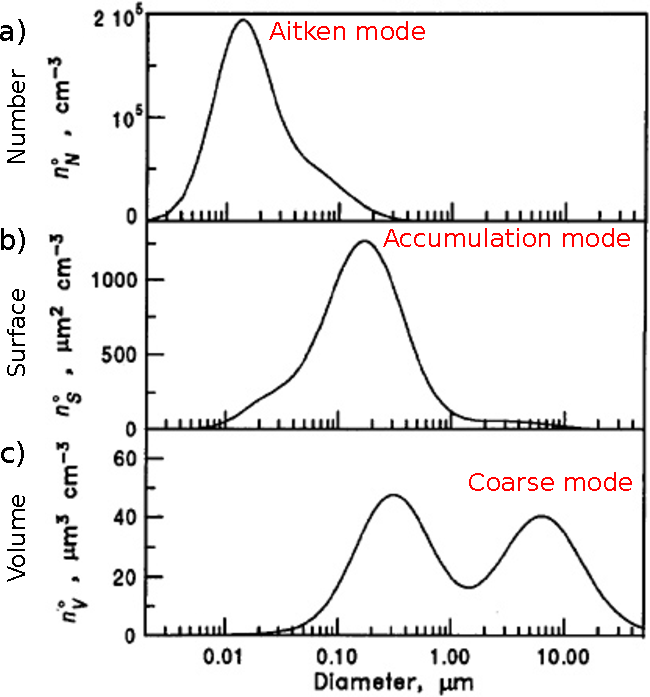
\includegraphics[width=0.4\textwidth]{aerosolDistribution.pdf}
    \caption{\textbf{(a)} Aerosol number, \textbf{(b)} surface area, and
        \textbf{(c)} volume for a typical trimodal aerosol
        distribution.  Figure adapted from the
    book of~\textcite{seinfieldAtmospheric1998}.}
    \label{fig:aerosolDistribution}
\end{figure}

An aerosol is composed of several chemical species like ions (\SOq, \NOt, \ce{Na+},
\ce{Cl-}, \ce{Mg^2+}, etc), metals (\ce{Cu}, \ce{Al}, \ce{Ti}, \ce{Ca}, etc), and organics species
(cellulose or other sugar, \og black carbon\fg, hopanes, etc).  They come from different
sources: natural like volcano, biology, desert (resuspension due to the wind) or marine
spray for instance and anthropogenic like traffic exhaust, brake wear, industry, biomass
burning or agriculture.  Each of these sources emits different species, in different
quantity and in different place of the atmosphere and of the Earth and with different
shape as shown in fig.~\ref{fig:micrography}.  However, the average lifetime of an aerosol
is from hour to week, and then can impact a wide area.  For instance the black carbon
emitted in developed countries is a major issue for the ice melt in the Artic's iceshelf.
More generally, aerosols are a key parameter in the climate system as they interact with
the Solar and Earth radiation, act as cloud/ice condensation nucleii and sectionicipate to
the precipitation process \autocite{boucherClouds2013}.

The nomenclature of the PM is linked to their size: \PMdix~covers all sectionicles with a
diameter lower than \SI{10}{\um}, \PMdc~with a diameter lower than \SI{2.5}{\um} and
\PMun~with a diameter lower than \SI{1}{\um}.  These categories do not have the same
chemical composition nor shape as they reflect different source or different process in
place in the atmosphere. Indeed, aerosols can react with the gas (\ce{SO2},
\ce{NO2}, \ce{NH3} for instance), radiation or radicals (the so call hydroxyl radical
\ce{HO^.}) or even with other aerosols and form new species or bigger aerosols. We then
call this aerosol \emph{secondary aerosol} as it do not reflect a primary source but
reaction in the atmosphere.

\begin{figure}[ht]
    \centering
    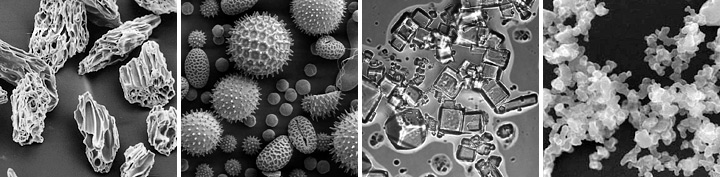
\includegraphics[width=1.0\textwidth]{aerosol_micrographs.jpg}
    \caption{Image au microscope electronique à balayage, à des échelles différentes,
        illustrant la diversité de forme des aérosols.
        De gauche à droite : cendre volcanic, polen, sel de mer et suie. Micrographies de
        l'USGS, UMBC (Chere Petty) et de l'Arizona State University (Peter Buseck). Credit
        : NASA earthobservatory
    \url{https://earthobservatory.nasa.gov/Features/Aerosols/}.}
    \label{fig:micrography}
\end{figure}

\subsection{Impacts climatiques des aérosols}%
\label{sub:impacts_climatiques_des_aerosols}
\paragraph{Noyaux de condensation}%
\label{par:noyaux_de_condensation}

\paragraph{Impact radiatif}%
\label{par:impact_radiatif}



\subsection{Impacts environnementaux}%
\label{sub:impacts_environnementaux}

\paragraph{Transport longue distance}%
\label{par:transport_longue_distance}


\paragraph{Polluants émergents}%
\label{par:polluants_emergents}



\subsection{Impacts sanitaires}%
\label{sub:impacts_sanitaires}



\section{Détermination des sources d'émission des PM}%
\label{sec:source_apportionment_of_pm}

\subsection{Signature chimique des sources d'émissions}%
\label{sec:chemical_signature_of_the_sources}

\subsection{Source apportionment model}%
\label{sec:source_apportionment_model}

\subsubsection{Direct modeling}%
\label{sub:direct_modeling}

\paragraph{Lagrangian or dispersion model}%
\label{sub:lagrangian_or_dispersion_model}

\paragraph{Deterministic chemistry transport model (CTM)}%
\label{sub:deterministic_chemistry_transport_model_ctm_}

\subsubsection{Receptor model}%
\label{sec:receptor_model}

\paragraph{Chemical mass balance (CMB)}%
\label{sub:chemical_mass_balance_cmb_}

\paragraph{Principal component analysis (PCA)}%
\label{sub:principal_component_analysis_pca_}

\paragraph{Positive matrix factorization (PMF)}%
\label{sub:positive_matrix_factorization_pmf_}


\section{Vers une mesure unifiée: le potentiel oxydant}%
\label{sec:le_potentiel_oxydant_des_aerosols}

Devant la grande variété de chimie, forme, taille, etc. des aérosols, il apparaît
compliqué de résumer la toxicité de l'air que l'on respire à sa simple concentration
massique en aérosols. En effet, il est évident que respirer un~\ugm{} de sable n'aura pas
le même impact sur notre santé qu'un~\ugm{} de mercure ou de plomb.
Seulement, la mesure massique est l'une des plus simples a implémenter en routine et est
également facilement automatisable, permettant ainsi un premier ordre de grandeur de 
l'exposition des populations. Aussi, il est important de rappeler que les aérosols n'ont
pas qu'un impacte sanitaire, mais également climatique (voir
section~\ref{sub:impacts_climatiques_des_aerosols}), pour lequel la messure de la concentration est tout a
fait adaptée.

Afin de répondre à ce problème, il a été proposé dans les années 2010 une nouvelle mesure,
intégratrice des propriétés physico-chimique des aérosols, sensé être plus proche des
impacte sanitaire occasioné par les PM. En effet, un des mécanismes suspecté d'être à
l'origine des troubles sanitaires engendrés par les aérosols est le stresse oxydatif
induit lors de l'inhalation des particules, entrainant une cascade de réaction au sain de
notre organisme.
Cette nouvelle mesure tente de quantifier les espèces réactive de l'oxygène (ROS) présente
ou induite par les aérosols en mettant en contact les aérosols et un antioxydant.
Le suivit de la cinétique de la réaction permet ainsi d'estimer la réactivité de la
particule, prenant en compte non seulement sa chimie, mais aussi la taille et forme des
particules à travers leurs surface de réaction et également les potentiels "effet
cocktail" lors de la combinaison de différentes espèces chimiques.

\subsection{Methodologie de mesure}%
\label{sub:methodologie_de_mesure}

\subsubsection{Prendre en compte la bioaccessibilité: SLF}%
\label{sub:prendre_en_compte_la_bioaccessibilite_slf}

\subsubsection{Differents agent réactant}%
\label{ssub:differents_agent_reactant}

\paragraph{Mesure par Ditiothreitol}%
\label{ssub:mesure_par_ditiothreitol}

\paragraph{Mesure par Acide ascorbic}%
\label{ssub:mesure_par_acide_ascorbic}

\paragraph{Mesure par DCFH}%
\label{ssub:mesure_par_dcfh}

\paragraph{Autres methodes de mesure}%
\label{sub:autres_methodes_de_mesure}

\subsubsection{Unitées de mesures}%
\label{ssub:unitees_de_mesures}

Mesure de réactivité par ug de PM ou par m3 d'air respirer.

\subsection{État de la connaissance du PO}%
\label{sub:etat_de_la_connaissance_du_po}



\addcontentsline{toc}{section}{Bibliography}
\printbibliography[segment=2,heading=subbibliography]
